\chapter{Højtaler \& Kabinet}

\section{Teori}
Højtaleren der benyttes til projektet er en 6.5" mellemtone elektrodynamisk højtaler af mærket FW168\cite{FW168} fra firmaet Fountek \cite{Fountek}.

\section{Simulering}

\newpage
\section{Realisering}
Højtalerens og kabinettets frekvenskarakteristik blev målt ved hjælp af en såkaldt CLIO Pocket. Der kan læses mere omkring dette værktøj og målemetoden i kapitel \ref{ch:measurements}; men det centrale er, at der måles på et frekvens-sweep (chirp). Der blev målt frekvensrespons på en lang række konfigurationer af højtaleren i forskellige miljøer og afstande.

I første omgang blev højtalerkabinettet placeret i det lyddøde rum således, at rummets egen frekvenskarakteristik blev nedsat og den målt frekvenskarakteristik derfor nærmede sig højtalerens egen frekvenskarakteristik.

\subsection{Lukket kabinet}
I denne konfiguration blev alle basrefleks-huller forseglet med propper således, at kabinettet var så godt som lufttæt. Frekvenskarakteristikken blev herefter målt ved, at placere CLIO-mikrofonen lige foran membranen og i 1 meters afstand foran membranen. Resultatet af dette ses på figuren nedenfor.
\begin{figure}[H]
	\centering
	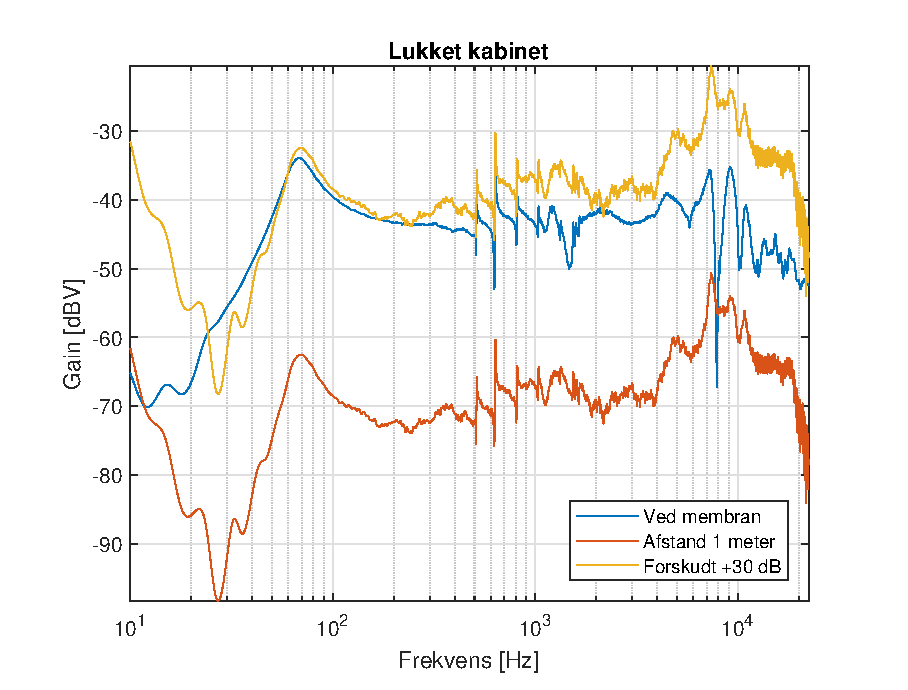
\includegraphics[width=\textwidth]{Pics/Graph}
	\caption{Målinger på et lukket kabinet}
\end{figure}

Det ses på figuren at, den første resonansfrekvens $f_s$ ligger ved omkring \SI{70}{\hertz} og at forstærkningen stiger med omkring 18 dB/oktav i det fjederstyrede område. Den målte resonansfrekvens stemmer ikke overens med 

Det ses også, at når CLIO-mikrofonen flyttes længere væk fra membranen, så bevarer karakteristikken sin form, men bliver forskudt nedad på y-aksen.